\subsection{Zielsetzung und architektonische Anforderungen}
Der Stand der Technik aktueller Simulationsplattformen für Roboter zeigt, dass
virtuelle Steuerungen und damit zusammenhängende Simulationsplattformen
herstellerspezifisch entwickelt und mit Ausnahme von ROS keine einheitliche
Schnittstelle zur Kommunikation mit externen Plattformen oder Physik-Engines
bieten. Somit muss für jeden Robotertyp ein designierter Konnektor genutzt
werden, um diesen mit einer externen, herstellerunabhängigen Simulationplattform
zu verbinden. Um eine herstellerunabhängige und erweiterbare Plattform zu
entwickeln, sollte also eine gemeinsame Schnittstelle implementiert werden.

Zusammenfassend verfolgt die Architektur des Frameworks drei zentrale
Ziele:

\begin{enumerate}
	\item \textbf{Vendor-Agnostik}: Abstraktion verschiedener Roboterhersteller durch einheitliche Interface-basierte Architektur ohne herstellerspezifische Abhängigkeiten im Kern-Framework

	\item \textbf{Modulare Erweiterbarkeit}: Plugin-System für Safety Monitoring Module und Kommunikationsprotokolle ohne Änderungen der bestehenden Architektur

	\item \textbf{Echtzeitfähige Kommunikation}: Latenzarme Datenübertragung für Motion Control und ereignisbasierte Sicherheitsüberwachung
\end{enumerate}

\subsection{Unity3D als Simulationsplattform}

\subsubsection{Auswahl und Vorteile gegenüber Alternativen}

Die Wahl von Unity3D als zugrundeliegende Simulationsplattform basiert auf
mehreren technischen und praktischen Erwägungen. Während es bereits mehrere
kommerzielle Programme für die Gestaltung und Simulation von Robotern in
virtuellen Umgebungen gibt, sind diese nur selten mit anderen CAD-Systemen und
Robotern kompatibel, unterstützen nicht alle Roboterbibliotheken oder werden
nur plattformabhängig angeboten (vgl. \vglcite[247]{andaluz2016}). Unity3D
hingegen ist mit den meisten CAD-Systemen kompatibel und bietet eine
plattformübergreifende Lösung.

\subsubsection{3D-Rendering und Physik-Simulation}

Unity3D bietet eine ausgereifte 3D-Rendering-Pipeline mit integrierter
Physik-Engine, welche zur Simulation von Gegenständen mit realitätsnahem
Verhalten sowie komplexen Arbeitsräumen geeignet ist (vgl.
\vglcite{Unity2025SystemRequirements}, \vglcite{Unity2025PhysicsOverview}). Die
Engine wurde bereits erfolgreich in der wissenschaftlichen Forschung eingesetzt
und bietet Module und Plugins für spezifische Anwendungsfälle im
Simulationsbereich. Unity3D ermöglicht es auch Nicht-Programmierern,
leistungsstarke Animations- und Interaktionsdesign-Tools zu nutzen, um Roboter
visuell zu programmieren und zu animieren (vgl. \vglcite[431]{bartneck2015}).

\subsubsection{Technische Architektur und Programmierung}

Technisch ermöglicht Unity3D durch seine Scripting-Runtime (basierend auf
Mono/.NET Framework) die Verwendung moderner C\#-Sprachfeatures für
nebenläufige Prozesse und asynchroner Programmierung
\vglcite[S.~45-52]{unity_async_2023}, was es ermöglicht, Visualisierung,
Datenakquise und Überwachung zu trennen. Die .NET-basierte Architektur
unterstützt dabei sowohl Task-basierte asynchrone Operationen als auch
Coroutines für zeitgesteuerte Prozesse
\vglcite[S.~123-135]{unity_coroutines_2023}, welche die notwendige periodische
Ausführung von Prozessen auf verschiedenen Ebenen des Frameworks stark
vereinfacht.

Die Unity-Engine unterstützt nativ Multithreading durch das Job System
\vglcite[S.~201-218]{unity_jobsystem_2023}, was für die parallele Verarbeitung
von Sensordaten, Kollisionserkennung und Bewegungsplanung entscheidend ist.

\subsubsection{Entwicklungsumgebung und Debugging-Tools}

Ein weiterer entscheidender Vorteil für die Robotik-Simulation liegt in der
Verfügbarkeit visueller Programmiertools und der integrierten
Entwicklungsumgebung. Die Plattform bietet umfangreiche Debugging- und
Profiling-Werkzeuge (Unity Profiler, Frame Debugger), die während der
Entwicklung und zur Laufzeit genutzt werden können
\vglcite[S.~67-89]{unity_profiler_2023}. Diese Werkzeuge ermöglichen die
Analyse von Performance-Engpässen bei der Verarbeitung von Roboterdaten und die
Optimierung der Sicherheitsmonitor-Updates.

Darüber hinaus lassen sich während der Laufzeit sowohl die Szene (hier: die
Roboterzelle) als auch Komponenten-Parameter in Echtzeit bearbeiten und
einsehen \vglcite[S.~1236]{haas_realtime_2022}, was das Debuggen und Testen
beschleunigt.

\subsubsection{Benutzerfreundlichkeit und industrielle Anwendung}

Besonders relevant für industrielle Robotik-Anwendungen ist die Möglichkeit,
Custom Editor Scripts zu entwickeln (vgl.
\vglcite[S.~156-172]{unity_editors_2023}), die eine benutzerfreundliche und
niederschwellige Konfiguration verschiedener Parameter ermöglichen. Zusätzlich
ermöglichen Gizmos und Scene View die visuelle Darstellung von Kollisionszonen,
Singularitätspunkten und Prozessabläufen während der Entwicklung (vgl.
\vglcite[S.~234-245]{unity_gizmos_2023}).

\subsection{Design Patterns und Prinzipien}

Die Entwicklung eines modularen und erweiterbaren Robotersicherheitssystems
erfordert eine fundierte methodische Herangehensweise, die auf bewährten
Software-Engineering-Prinzipien basiert. Die Auswahl geeigneter Design Patterns
und Architekturprinzipien determiniert maßgeblich die Qualitätsattribute des
Systems wie Wartbarkeit, Testbarkeit und Erweiterbarkeit (vgl.
\vglcite{Bass2012}, S. 73-75). Im Folgenden werden die für diese Arbeit
gewählten Entwurfsmuster und deren Begründung dargelegt.

\subsubsection{Observer Pattern als Kommunikationsparadigma}
Für die Realisierung der systemweiten Kommunikation wird das Observer Pattern
(vgl. \vglcite{Gamma1994}, S. 293-303) als zentrales Entwurfsmuster gewählt.
Diese Entscheidung basiert auf drei wesentlichen Anforderungen industrieller
Robotersysteme: Erstens müssen Sicherheitsereignisse ohne Verzögerung an alle
relevanten Systemkomponenten propagiert werden, was durch die inhärente
Entkopplung des Observer Patterns gewährleistet wird. Zweitens ermöglicht das
Muster die dynamische Registrierung und Deregistrierung von Beobachtern zur
Laufzeit, was für modulare Sicherheitssysteme unerlässlich ist (vgl.
\vglcite{Buschmann1996}, S. 127-128). Drittens reduziert die lose Kopplung
zwischen Publisher und Subscriber die Systemkomplexität erheblich, da
Komponenten ohne Kenntnis voneinander interagieren können.

Das Observer Pattern adressiert zudem die Herausforderung der
Multi-Threading-Umgebung in Unity3D, indem Events asynchron verarbeitet werden
können, ohne den Hauptthread zu blockieren (vgl. \vglcite{Nystrom2014}, S.
156-159). Dies ist besonders kritisch für die Echtzeitverarbeitung von
Sensordaten und die gleichzeitige Visualisierung.

\subsubsection{Strategy Pattern für algorithmische Flexibilität}
Die Wahl des Strategy Patterns (vgl. \vglcite{Gamma1994}, S. 315-323) für die
Implementierung von Sicherheitsmonitoren und Datenparser begründet sich durch
die Heterogenität industrieller Robotersysteme. Verschiedene Roboterhersteller
verwenden proprietäre Kommunikationsprotokolle und Datenformate, was eine
flexible Austauschbarkeit von Parsing-Algorithmen erfordert (vgl.
\vglcite{Siciliano2016}, S. 891-893). Das Strategy Pattern kapselt diese
Algorithmen in separaten Klassen und macht sie über eine gemeinsame
Schnittstelle austauschbar.

Die Vorteile dieser Architekturentscheidung manifestiert sich vornehmlich
darin, dass so Robotertypen ohne Modifikation des Kernsystems integriert
werden. \textsc{Martin2003} spricht hier vom Open-Closed-Prinzip, welches die
Offenheit von Software-Entitäten (Funktionen, Klassen, Module, Komponenten
usw.) zur Extension und die gleichzeitige Geschlossenheit zur Modfikation
beschreibt.\vglcite{Martin2003}

\subsubsection{Adapter Pattern zur Hardware-Abstraktion}
Die Integration heterogener Hardware-Komponenten erfordert eine
Abstraktionsschicht zwischen der Anwendungslogik und den hardware-spezifischen
Schnittstellen. Das Adapter Pattern (vgl. \vglcite{Gamma1994}, S. 139-150) wird
gewählt, um diese Abstraktion zu realisieren. Die Notwendigkeit ergibt sich aus
der Vielfalt der Robotersteuerungen und Visualisierungssysteme, die jeweils
eigene APIs und Datenformate verwenden (vgl. \vglcite{Craig2005}, S. 412-415).

Durch die Adapter-Schicht wird eine einheitliche Schnittstelle zur Verfügung
gestellt, die es ermöglicht, verschiedene Robotersysteme ohne Änderung der
Kernlogik anzubinden. Dies reduziert nicht nur die Komplexität des Systems,
sondern erhöht auch dessen Portabilität und Wiederverwendbarkeit (vgl.
\vglcite{Vlissides1995}, S. 89-91).

\subsubsection{SOLID-Prinzipien als Qualitätsfundament}
Die konsequente Anwendung der SOLID-Prinzipien (vgl. \vglcite{Martin2003}, S.
95-135) bildet das methodische Fundament der Systemarchitektur. Das
\textit{Single Responsibility Principle} wird angewendet, um kohäsive Module zu
schaffen, die genau eine Verantwortlichkeit haben. Dies reduziert die Kopplung
und erhöht die Verständlichkeit des Codes (vgl. \vglcite{Martin2017}, S.
62-64). Das \textit{Open-Closed Principle} gewährleistet, dass das System für
Erweiterungen offen, aber für Modifikationen geschlossen ist – eine essenzielle
Eigenschaft für langlebige Industriesysteme.

Das \textit{Dependency Inversion Principle} wird konsequent angewendet, indem
High-Level-Module von Abstraktionen abhängen, nicht von konkreten
Implementierungen. Dies ermöglicht die flexible Konfiguration des Systems zur
Laufzeit und vereinfacht die Integration in verschiedene Produktionsumgebungen
(vgl. \vglcite{Fowler2018}, S. 112-115).

\subsubsection{Event-Driven Architecture für Echtzeitfähigkeit}
Die Entscheidung für eine event-getriebene Architektur basiert auf den
Echtzeitanforderungen industrieller Robotersysteme. Sicherheitskritische
Ereignisse müssen innerhalb definierter Zeitschranken verarbeitet werden, was
durch synchrone Aufrufketten nicht gewährleistet werden kann (vgl.
\vglcite{Hohpe2003}, S. 97-99). Die event-getriebene Architektur ermöglicht die
asynchrone Verarbeitung von Ereignissen und die Priorisierung kritischer
Sicherheitsereignisse.

Zudem adressiert dieser Ansatz die Herausforderung der Integration
verschiedener Datenquellen – von zyklischen Sensordaten über sporadische Alarme
bis zu kontinuierlichen Videoströmen. Jede Datenquelle kann Events in ihrem
eigenen Takt generieren, ohne andere Systemkomponenten zu blockieren (vgl.
\vglcite{Vernon2013}, S. 234-237).

\subsection{Systemarchitektur und Entwurfsmuster}

\subsubsection{Flange Framework als Visualisierungs- und Konfigurationstool}
Im Rahmen dieses Frameworks wird das Unity-Package
\textit{Flange} genutzt. Implementiert durch GitHub-User \textit{Preliy} und frei
verfügbar im Rahmen einer BSD 3-Clause Lizenz, bietet ein spezialisiertes
Framework für die Robotersteuerung in Unity mit modularer Architektur, die
Gelenksteuerung, Kinematik, Koordinatentransformationen und Echtzeitüberwachung
als separate Komponenten organisiert. Das System unterstützt sowohl direkte
Gelenkmanipulation auf niedriger Ebene als auch kartesische Steuerung auf
höherer Abstraktionsebene, wodurch es für verschiedene Roboteranwendungen
einsetzbar ist.\vglcite{preliyflange2024} Im Kontext dieser Entwicklungsarbeit wird Flange zur
Implementierung und Visualisierung der Denavit-Hartenberg-Parameter und damit
einhergehender Achstransformationen eingesetzt,
da diese Notation als fundamentales Werkzeug der Robotik eine systematische
Beschreibung der Geometrie serieller Robotermechanismen ermöglicht und somit die
Anwendung etablierter algorithmischer Verfahren für kinematische Berechnungen,
Jacobi-Matrizen sowie Bewegungsplanung unterstützt.\vglcite[590]{corke2007}

Flange ermöglicht eine direkte Konfiguration des Roboters über \textit{Frame}
und \textit{JointTransformation} Scripts. Ein Frame definiert dabei die
Denavit-Hartenberg-Parameter für einen Teil der kinematischen Kette, eine
JointTransformation die Paramter des Gelenks, also möglicher maximaler Ausschlag
in positive und negative Achsrotationsrichtung sowie maximale Geschwindigkeit
und Beschleunigung. Diese Funktion werden im Rahmen dieser Implentierung
genutzt, um den zu simulierenden Roboter theoretisch nachvollziehbar im Raum
bewegen zu können.

\subsubsection{Schichtenarchitektur}
Aufbauend auf den oben genannte Prinzipien teilt sich das Framework in 4
logisch getrennte Module auf:
\begin{enumerate}
	\item \textbf{Kernlogik}, welches den Status des Roboters beinhaltet und verwaltet als
	      zentrale Schnittstelle (Core)
	\item \textbf{Interfaces}, welche die Kommunkationsschnittstellen und -methoden
	      zwischen den Modulen implementiert (Interfaces)
	\item \textbf{Monitoring}, welches die einzelnen Komponenten des Monitoring-Systems
	      implementiert (Monitors)
	\item \textbf{Adapters}, welches potenziell Adapter zu veschiedenen physischen oder
	      simulierten Steuerungen von Robotern beinhaltet (Hier ABB gennant)
\end{enumerate}
Beispielhaft wird im Folgenden erläutert, aus welchen Bestandenteilen Interfaces
des Framework bestehen. Da jedes Modul, welches von einer Interface erbt
zwangsweise dessen Komponenten implenentieren muss, lassen sich hierdurch die
grundlegenden Funktionalitäten des Framework abstrahieren.

\subsubsection{Interfaces}
Die Trennung der Module ermöglicht eine formalisierte
Schnittstellenkommunikation, dargestellt in Abbildung \ref{figure:layer}.
Jede Schicht hat verschiedene Verantwortlichkeiten und
Schnittstellen innerhalb des Monitoring-Systems. Die Robot Communication Layer
organisiert die Kommunkation mit der zugrundeliegenden Robotersteuerung und
implentiert eine Interface des Typs IRobotConnector. Als Verbindungsclient
zwischen Unity und externer Schnittstelle des Robotersystems implementiert
dieser eine IRobotConnector Interface, welche als Vorlage für eine Anbindung an
eine Robotersteuerung jedes Typs fungiert und standartisierte Methoden
implementiert:
\begin{lstlisting}  
namespace RobotSystem.Interfaces
{
    public interface IRobotConnector
    {
        event System.Action<RobotSystem.Core.RobotState> OnRobotStateUpdated;
        event System.Action<bool> OnConnectionStateChanged;
        
        bool IsConnected { get; }
        RobotSystem.Core.RobotState CurrentState { get; }
        
        void Connect();
        void Disconnect();
    }
}
\end{lstlisting}
Eine Interface lässt sich anhand dieses Beispiels in 3 Funktionsbereich aufteilen: Events, Attribute und Methoden.

Die Interface definiert Events (Aktionen), die bei definierten Zustandsänderungen
in der Laufzeit ausgeführt werden. Andere Bestandteile des Framework sind in der
Lage, ein Event zu abonnieren und eine Methode registieren, welche ausgeführt
werden soll, wenn dieses Event auftritt. Ist dies der Fall, wird das
entsprechende Modul über die Änderung benachrichtigt und bekommt gegebenfalls
neue Daten zur Verfügung gestellt. Diese event-getriebene Kommunikation sorgt
dafür, dass einerseits alle Komponenten proaktiv auf den neusten Stand der Daten gebracht
und gehalten werden, andererseits aber keine ressourcenblockierenden Prozesse
ausgeführt werden müssen, um gegebenfalls Statusänderungen abzufragen.

Weiterführend definiert die Interface IRobotConnector Attribute, welche den
aktuellen Verbindungsstatus (verbunden=true, getrennt=false) speichern sowie das
State-Objekt des Roboters. Definiert durch die schreibgeschützten, automatisch
implementierte Eigenschaft mit einem Getter \textit{\{ get; \}} können Attribute
auch von ausserhalb des RobotConnectors abgefragt werden, jedoch nicht
überschrieben.


Zuletzt gibt die Interface die Methoden \textit{Connect} und \textit{Disconnect}
vor, welche hier die wichtigsten Methoden zum Verbinden und
Trennen von der jeweiligen Robotersteuerung darstellen.

\begin{figure}[htbp]
	\centering
	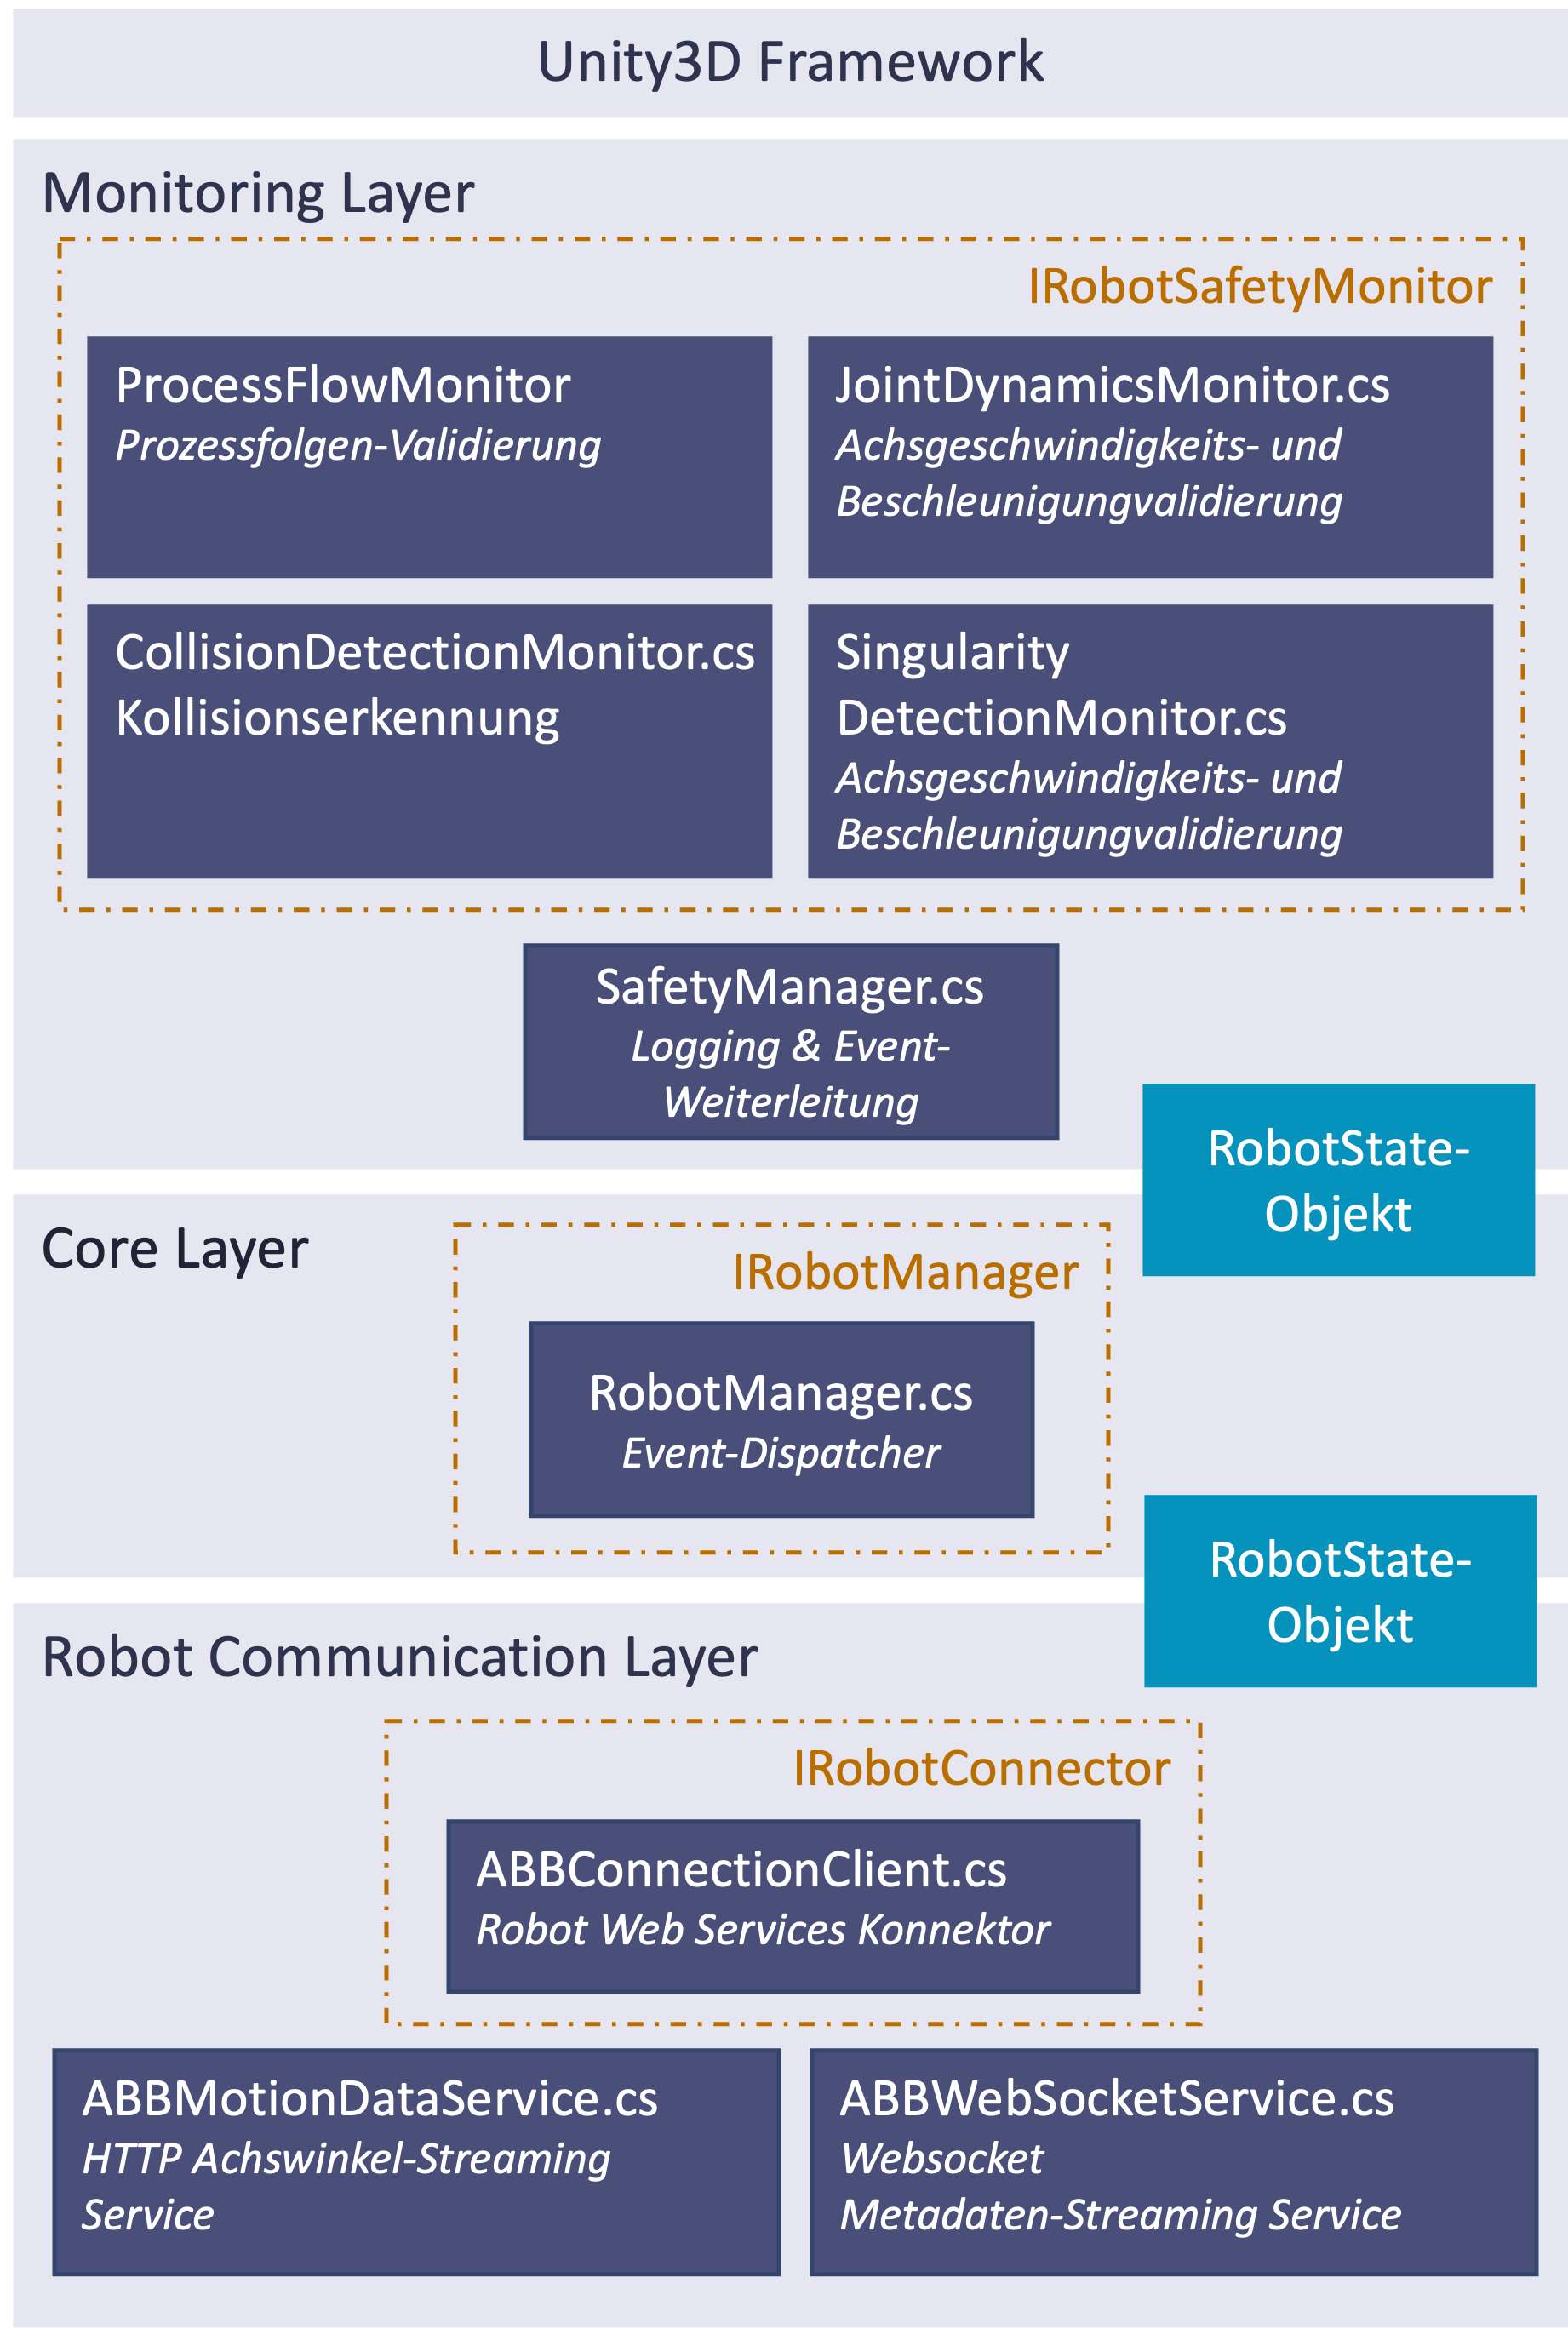
\includegraphics[width=10cm]{Figures/LayerArchitekturFramework.png}
	\caption{Schichtenarchitektur des Frameworks mit den wichtigsten zugehörigen
		Modulen. Module mit grüner Umrandung werden durch ine Interface formalisiert.}
	\label{figure:layer}
\end{figure}

\dirtree{%
	.1 RobotSystem/.
	.2 Core/.
	.3 RobotManager.cs.
	.3 RobotState.cs.
	.3 RobotSafetyManager.cs.
	.3 SafetyEvent.cs.
	.3 RobotStateSnapshot.cs.
	.3 Part.cs.
	.3 Station.cs.
	.3 RapidTargetGenerator.cs.
	.2 Interfaces/.
	.3 IRobotConnector.cs.
	.3 IRobotDataParser.cs.
	.3 IRobotSafetyMonitor.cs.
	.3 IRobotVisualization.cs.
	.2 ABB/.
	.3 RWS/.
	.4 ABBRWSConnectionClient.cs.
	.4 ABBRWSDataParser.cs.
	.4 ABBMotionDataService.cs.
	.3 ABBFlangeAdapter.cs.
	.2 Monitors/.
	.3 CollisionDetectionMonitor.cs.
	.3 JointDynamicsMonitor.cs.
	.3 ProcessFlowMonitor.cs.
	.3 SingularityDetectionMonitor.cs.
}

\paragraph{Event-Driven Architecture}
Das System nutzt ein durchgängiges Event-System für lose Kopplung:
\begin{itemize}
	\item \texttt{OnRobotStateUpdated}: Zustandsänderungen
	\item \texttt{OnConnectionStateChanged}: Verbindungsstatus
	\item \texttt{OnSafetyEventDetected}: Sicherheitsereignisse
	\item \texttt{OnMotorStateChanged}: Motorstatusänderungen
\end{itemize}

\paragraph{SafetyEvent und RobotStateSnapshot}
Das \texttt{SafetyEvent}-System implementiert ein umfassendes Ereignismodell:
\begin{itemize}
	\item \textbf{SafetyEvent}: Unveränderliches Value Object für Sicherheitsereignisse
	\item \textbf{RobotStateSnapshot}: Immutable Zustandserfassung zum Ereigniszeitpunkt
	\item \textbf{Ereignistypen}: Info, Warning, Critical mit konfigurierbaren Schwellwerten
	\item \textbf{Kontextdaten}: Vollständige Roboterzustandserfassung für Forensik
\end{itemize}

\paragraph{Datenformate}
\begin{itemize}
	\item \textbf{HTTPS/HTTP}: RESTful API-Zugriff mit Digest-Authentifizierung
	\item \textbf{WebSocket Secure (WSS)}: Bidirektionale Echtzeit-Kommunikation
	\item \textbf{XML}: Strukturierte Datenübertragung mit Schema-Validierung
	\item \textbf{JSON}: Interne Datenrepräsentation und Logging-Format
\end{itemize}

as
